\clearpage
\section{Literature}

\subsection{Multimodal Machine Learning}

We experience the world as multimodal: we see objects, feel vibrations and hear sounds. Modality refers to the way in which something happens or is experienced. A research problem is characterized as multimodal when it includes multiple of such modalities \cite{Baltrusaitis2017}. Commonly referred example of an interesting multimodal experience is the McGurk effect \cite{McGurk1976}. This is the perception between hearing and vision in speech. When we hear the syllable /ba/ while watching the lips of someone saying /ga/, we perceive it as /da/. 

Multimodal research has a long history from audio-visual speech recognition to more recent interest due deep learning \cite{Ngiam2011}. It has been proven that multimodal learning algorithms performs really well on various tasks, such as (audio-visual) speech recognition \cite{Noda2014}, image sentence matching \cite{Ma2015} and RGB-D object recognition \cite{Eitel2015,Xu2017,Sindagi2019}.

\authorref{Baltrusaitis2017} identified five challenges dealing with multimodal machine learning:
\begin{enumerate}
\item \textbf{Representation}: how to represent and summarize multimodal data to exploit the complementary and redundancy of multiple modalities. Distinction is made between \textit{joint representation} - which combines unimodal signals in the same space, and \textit{coordinated representation} - which processes unimodal signals separately, but enforces similarity constraints. See figure \ref{fig:structure-joint-coordinated} below for an illustration.
\item \textbf{Translation}: how to translate data from one modality to another. For example, given an image the task is to give a caption to describe the image.
\item \textbf{Alignment}: how to identify direct relations between (sub)elements from multiple modalities. For example, given an image and a caption, find the area in the image describing the caption.
\item \textbf{Fusion}: how and when to fuse / join information from multiple modalities. Historically the original topics of multimodal machine learning, with emphasize given on early-, hybrid- and late-fusion.
\item \textbf{Co-learning}: how to transfer knowledge between modalities. For example by exploiting knowledge of a rich modality, to aid modelling of a less describing modality.
\end{enumerate}

\begin{figure}[ht]
\begin{center}
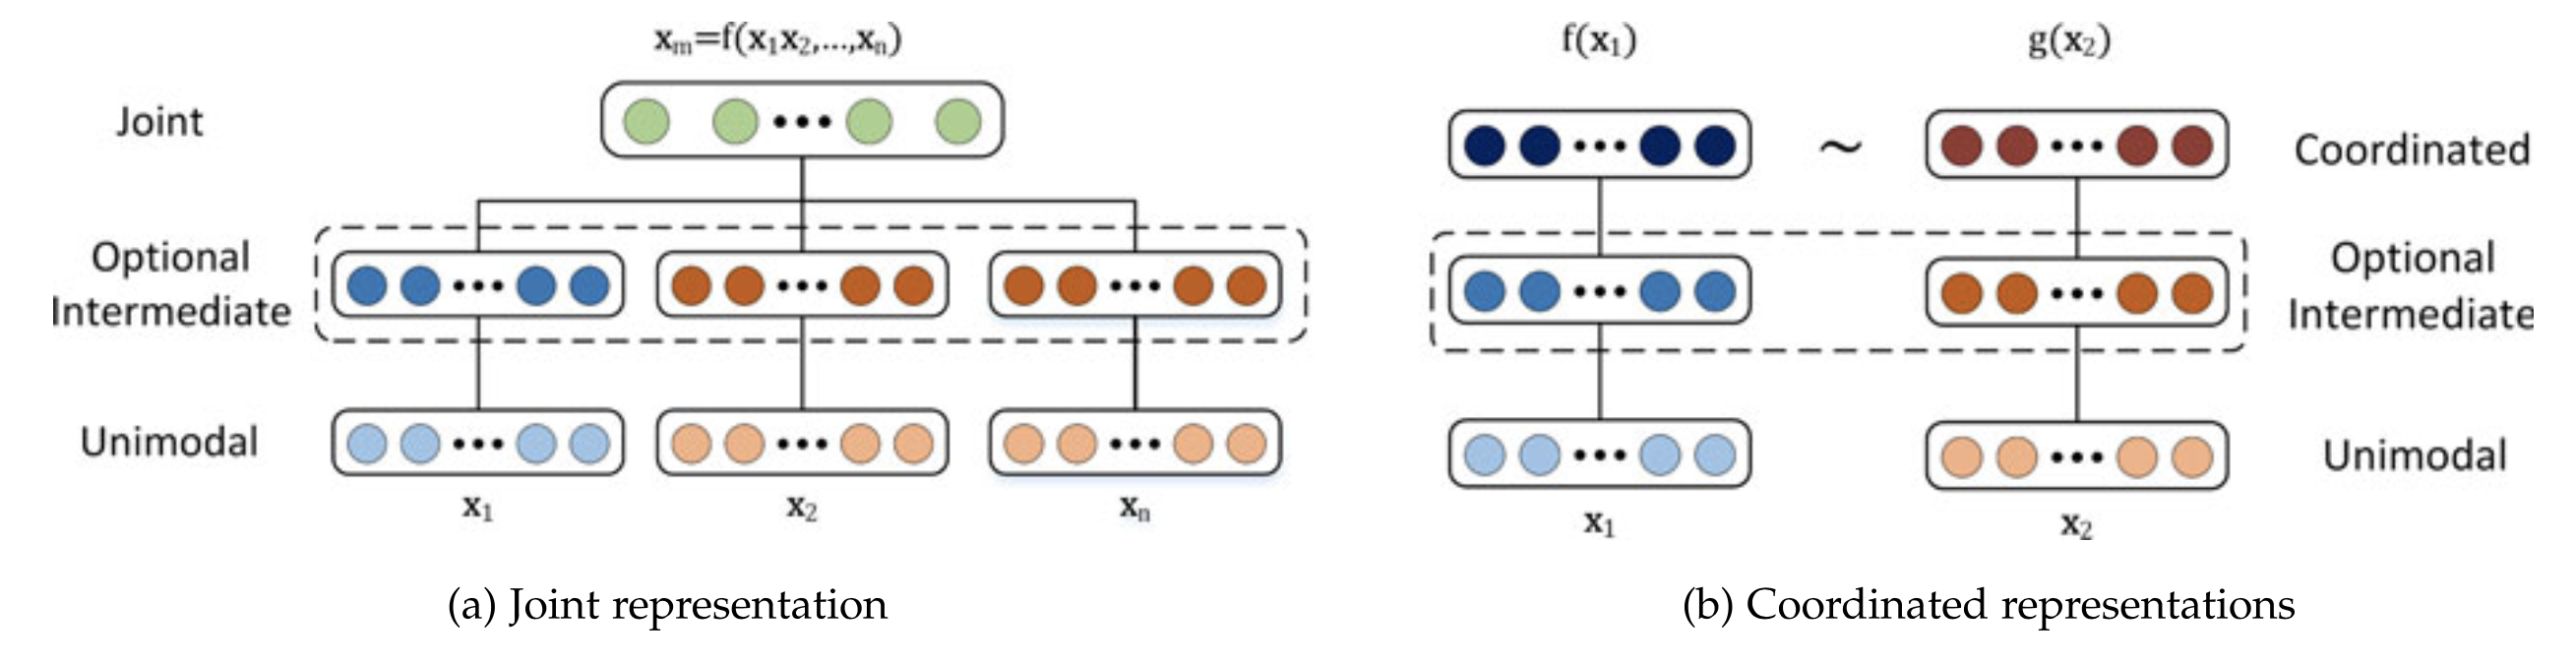
\includegraphics[width=\textwidth,keepaspectratio]{images/2_literature/joint-vs-coordinated-representations.png}
\end{center}
\caption{Structure of joint and coordinated representation \cite{Baltrusaitis2017}}
\label{fig:structure-joint-coordinated}
\end{figure}

For my thesis I think the most important challenges will be relating to representation, alignment and fusion.

To my knowledge there hasn't been any research performed on multimodal fusion on road defects. In the broader sense, multimodal fusion has been applied to detect damages. Examples of which are: combining audio-visual data to detect conveyor belt damages \cite{Che2021}, gearbox fault detection based on vibrations and acoustic signals \cite{Li2016}. See \cite{Olivan2018} for more examples of data fusion in industry.

Further exploratory research shows that visual and accelerometer (IMU) data are mainly fused in odometry. Odometry is the use of motion sensors to estimate the location over time, often used in intelligent robots. The purpose of fusing these data types is often used for dead-reckoning. Which is the process of calculating the current position based on previously known position, e.g. can be used when GPS connection is unstable / lost \cite{Jiang2017,Brossard2020}.

Although mutimodal fusion hasn't been applied to road surface defects, something related has been done by \authorref{Lekshmipathy2020}. In the paper the researchers compared the results of classifying defects based on vibrations (accelerometer) with a vision-based method. They find that vision-based method outperforms the vibration-based method. Nevertheless, they argue that vibration-based method is still useful. Vision based approach only works during daytime (under correct lighting), whereas vibrations can always be collected regardless of lighting situation or weather.

\subsubsection{Conclusion}
Although multimodal machine learning is not something new, it hasn't been applied in the domain of road maintenance. To my knowledge the fusion of accelerometer and visual data hasn't been used yet for detecting damages in general. The closest comes the work of \authorref{Lekshmipathy2020}, where they compare vibration- and visual-method for classifying road defects. My thesis aims to fill the gap by applying multimodal machine learning to detect road damages. 

% ********************************************************************************
% ********************************************************************************
% ********************************************************************************

\subsection{Automatic Road Defects Classification}

Preliminary literature review shows that there is a whole field about data driven road quality assessment. This field is driven by the fact that traditional methods of assessing road quality is costly, due requirement of specialized equipment. Researchers focuses on alternative forms to collect the data by cheaper methods, such as smartphones and sensor boxes. In current literature we identified the following \textit{subfields} based on the type of data that is used:

\begin{enumerate}
\item Road surface defects: based on image data (e.g. cracks).
\item Roughness evaluation: based on accelerometer / gyroscope (e.g. IRI).
\item Noise labelling: based on microphones.
\end{enumerate}

\begin{figure}[h!]
\begin{center}
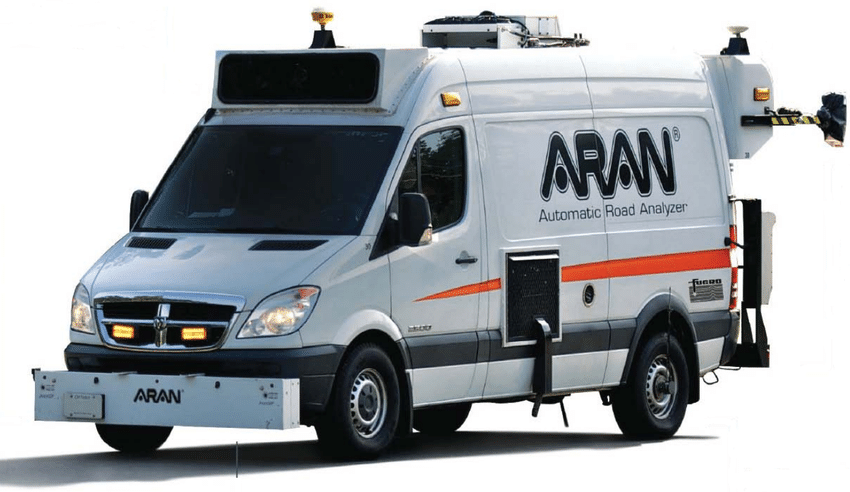
\includegraphics[height=5cm,keepaspectratio]{images/2_literature/aran.png}
\end{center}
\caption{Automatic Road Analyzer (ARAN) is specialized vehicle to gather data about the road surface \cite{Gupta2020}.}
\end{figure}

\subsubsection{Road surface defects}
Road surface defects or crack detection is a field trying to automatically classify damages based on image data. Usually the source of these images are smartphones. Additionally, there is also research performed using blackboxes (dashcams) and Kinect, where the latter is also able to measure depth. Research evolved from pictures taken from a top-down view, to front-faced view to support gathering data while driving.

In \authorref{Jahanshahi2012} the authors uses a Kinect sensor to collect image and depth data. Recording of the road has been performed from a top-faced view. The authors classify cracks, potholes and patches with accuracy scores of respective 78\%, 92\% and 90\%. By including depth measure, the problem is relatively trivial as classification is done by checking if the depth is greater than some threshold. 

\authorref{Zhang2016} proposes the first model (to their knowledge) which uses deep learning to detect road cracks. Their data has been collected by smartphones, although not mentioned explicitly, it seems their data has been collected from top-faced view and from deliberate pictures of a known defect. Related is \authorref{Zhang2017} where the authors use 3D pavement images and deep-learning network to classify road cracks. Their research is focused on acquiring pixel-level accuracy, with the aim that the model is able to tell the size and dimensions of the crack.

\authorref{Chatterjee2018} perform road crack detection on cycle roads in Germany. Their data has been collected from a front-faced view. Extensive feature extraction is performed with various computer vision based algorithms before making classifications with machine learning models. 

\authorref{Maeda2018} researched the possibilities of road damage classification by using smartphone images. Data was collected conventional smartphone holder for cars with a front-faced view while driving. They extensively collect data about Japanese roads and publishes their data and their trained model. This is also the first paper which makes distinctions between more types of road damages, such as fading line markings and distinction between lateral / longitudal cracks. The research is continued in \authorref{Arya2020-transfer}, where additional data is collected in Czech Republic and India. With the aim to see if their model is able to transfer learn on this new data. In order to further improve the published model, \authorref{Maeda2020} uses a generative adversial network to augment more data and retrain the model. Finally, a competition is held with their collected data \cite{Arya2020-competition}. The goal is to push the state of art of road damage detection forward. The competition consisted of two challenges: 1) classification (what kind of damage) and 2) detection (where is the damage). This competition yielded a model with an average F1 score of 0.67 for all classes. Greatly improving the original model, which yielded at best a F1 of 0.40 for only a single type of damage.

Besides making classifications, there has also been research focusing on segmenting the damages into crack and non-crack parts. \authorref{Dung2018} uses a fully convolutional neural network and \authorref{Bang2019} uses a encoder-decoder network.


\subsubsection{Roughness evaluation}
A different research field is centered around measuring the road roughness. Which is defined as the deviation of the surface from the true planar surface. This deviation affects vehicle dynamics and ride quality. Two methods to classify the roughness of a profile are the International Roughness Index (IRI) \cite{Sayers1986} and the International Standards Organisation (ISO) \cite{ISO8608} classification. There are various methods for measuring the profile data, typically used by road maintenance are inertial profilers. This is a device which scans the surface of the pavement with lasers to measure the distance, example of this is the Automatic Road Analyzers (ARAN) vehicle.

Research is focused on replacing these expensive devices with accelerometers, often those found in smartphones \cite{Hanson2014,Buttlar2014,Gupta2020}. Measuring the profile is done by filtering out the vertical accelerations and calculate the roughness accordingly to the IRI or ISO specification. Additionally, using the accelerometer it is also possible to identify potholes, bumps and patches \cite{Lekshmipathy2020}. 

Limitation of this method is that the accelerometers need to be calibrated, which is also deeper described in \cite{Gupta2020}. \authorref{Jeong2020} therefore argue that requirement of calibration hinders the widespread use of the technology. They propose a novel method using a convolutional neural network to eliminate the requirement of calibration.


\subsubsection{Noise labelling}
Quality of the road surface influences noise and vibrations emissions caused by the interaction between the tires and the road. In the EU, member states are required to publish noise maps for roads every five years \cite{EU2002}. Monitoring can be done with a vehicle equipped with a Close Proximity (CPX) trailer. This devices measures the emitted sounds from a reference tire.

\begin{figure}[ht]
\begin{center}
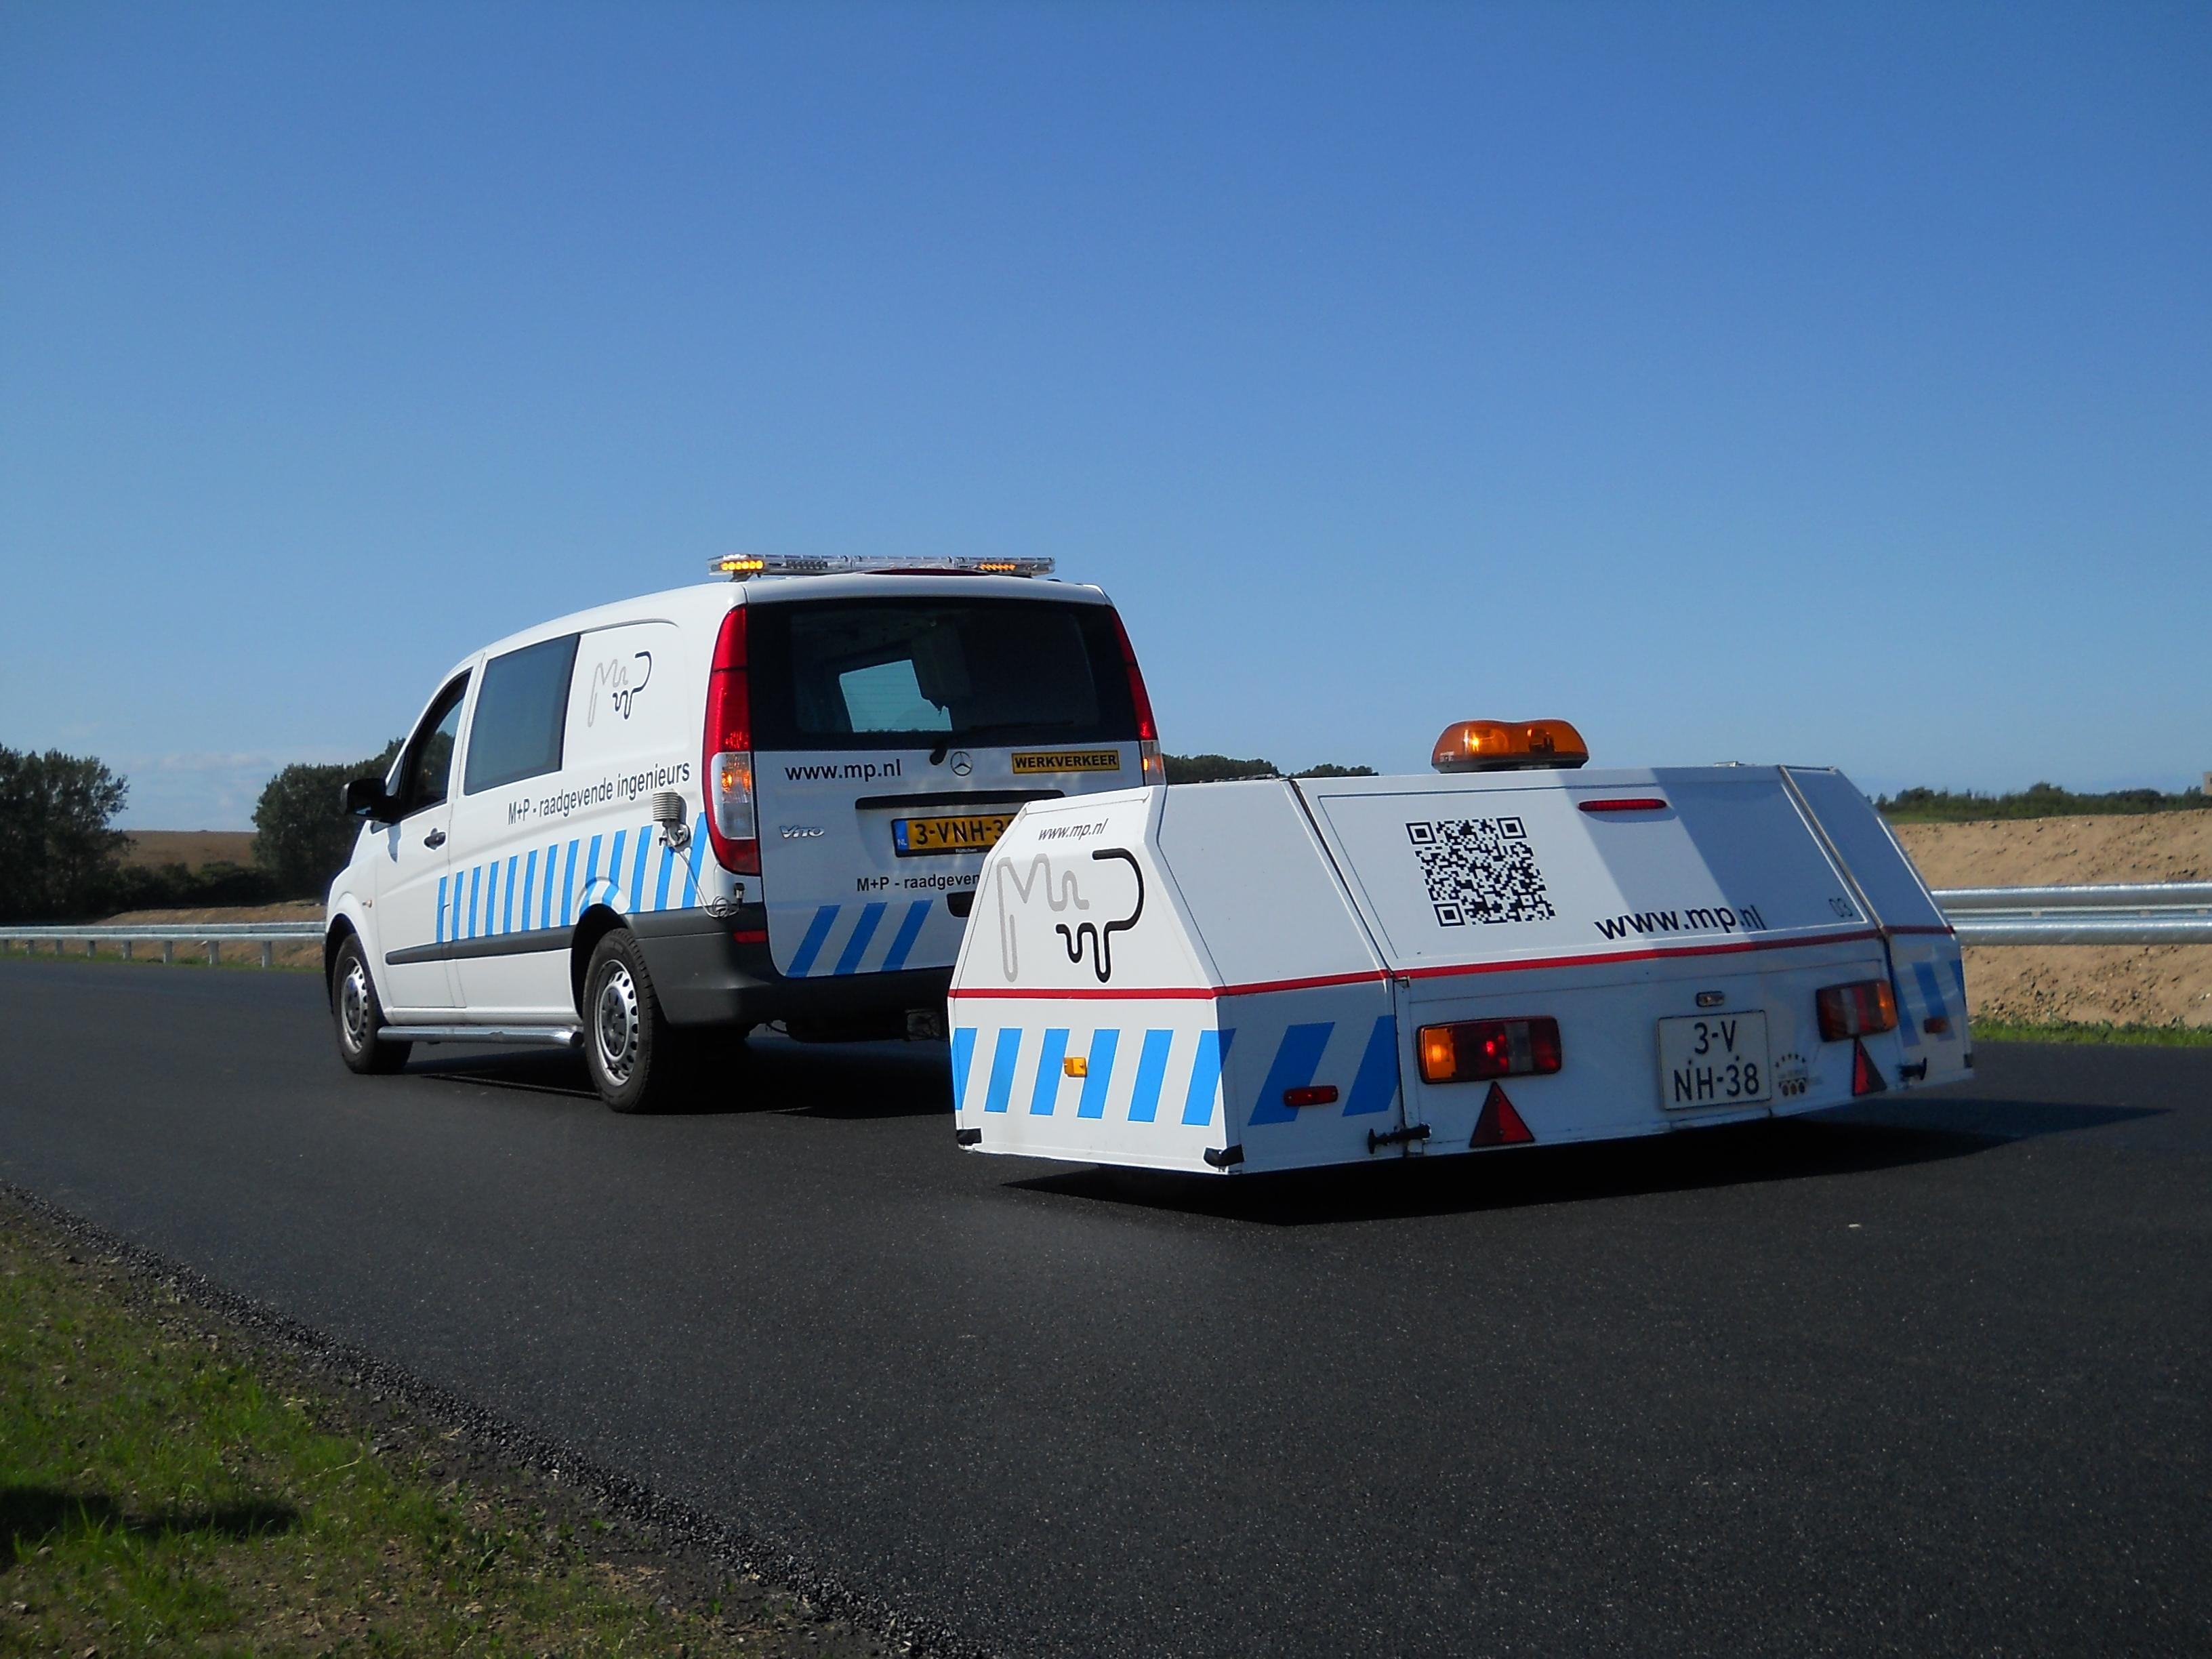
\includegraphics[height=5cm,keepaspectratio]{images/2_literature/cpx-trailer.jpg}
\end{center}
\caption{Close Proximity (CPX) trailer measures the sounds emitted by reference tyre \cite{MP2020}.}
\end{figure}

\authorref{Hauwermeiren2019} try to replicate the results of CPX measurements by using a sensor box containing a microphone. This microphone is located inside the trunk of the car. The authors were able to accurately estimate the road texture. However the with main limitation is that the data was collected under good conditions, such as no background radio or talking. This research is later continued, where the authors use multiple vehicles and more realistic driving conditions. They found that below 1600 Hz, their results differ from CPX less than the difference between bi-annually repeated measurements, indicating it is possible to perform this measurement using microphones \cite{Hauwermeiren2021}.


\subsubsection{Conclusion}
Automatic classification of road defects have been extensively researched. Main topic of interest is the usage of low-cost devices such as smartphones to collect the data. From the literature we find that only the following types of defects are classified: cracks, patches, holes and faded line markings. Raveling, rutting and skewed signs haven't been researched yet to my knowledge. From the field of classifying road defects we can draw a lot of knowledge to use for my thesis. Especially this is useful when to model the right representations of the data to use for multimodal machine learning.

% ********************************************************************************
% ********************************************************************************
% ********************************************************************************

\subsection{Object Detection}

% ********************************************************************************
% ********************************************************************************
% ********************************************************************************

\subsection{Accelerometer Signal Processing}

% ********************************************************************************
% ********************************************************************************
% ********************************************************************************

\subsection{Alignment of Sources in Multimodal Fusion}